%----------------------------------------------------------------------------------------
%	PACKAGES AND THEMES
%----------------------------------------------------------------------------------------
\documentclass[aspectratio=169,xcolor=dvipsnames,handout]{beamer}
\usetheme{Darmstadt}
\usecolortheme{seahorse}

\usepackage[hangul]{kotex}

\usepackage{hyperref}
\usepackage{graphicx} % Allows including images
\usepackage{booktabs, multicol, multirow} % Allows the use of \toprule, \midrule and \bottomrule in tables
\setbeamercovered{transparent}
%----------------------------------------------------------------------------------------
%	TITLE PAGE
%----------------------------------------------------------------------------------------

\title[후생경제학]{후생경제학} % The short title appears at the bottom of every slide, the full title is only on the title page
\subtitle{경제정의와 불평등}

\author[오성재]{오성재}

\institute[HNU] % Your institution as it will appear on the bottom of every slide, may be shorthand to save space
{
    한남대학교 \\
    탈메이지 교양학부 \\
}
\date{\today} % Date, can be changed to a custom date


%----------------------------------------------------------------------------------------
%	PRESENTATION SLIDES
%----------------------------------------------------------------------------------------

\begin{document}

\begin{frame}
    % Print the title page as the first slide
    \titlepage
\end{frame}

\begin{frame}{목차}
    % Throughout your presentation, if you choose to use \section{} and \subsection{} commands, these will automatically be printed on this slide as an overview of your presentation
    \tableofcontents
\end{frame}
%------------------------------------------------

\begin{frame}{경제학의 기본 문제}
        \centering
        {\bf \Large 주어진 자원은 희소한데 인간의 욕망은 무한하다.}
\end{frame}
%------------------------------------------------

%------------------------------------------------
\section{개인들의 의사결정}
%------------------------------------------------

\begin{frame}{개인의 선호체계(preference) 가정}
    \begin{itemize}
        \item  경제학의 대상인 개인들은 주로 아래의 특성을 가진 선호체계로 대표된다.
        \begin{itemize}
            \item 완비성 : 모든 대안에 대하여 선호가 존재.
            \item 단조성 : 다다익선.
            \item 이행성 : 사과 $\preceq$ 배 그리고 배 $\preceq$ 딸기 $\rightarrow$ 사과 $\preceq$ 딸기.
            \item 볼록성 : 극단보다는 중간을 선호.
            \item 서수적 효용 : 효용은 그 순서만이 중요. 개인간 효용비교를 하지 않음. 
        \end{itemize}
        \item 이상의 특성을 가진 개인은 자신의 효용의 크기를 숫자로 나타낼 수 있음.
    \end{itemize}
\end{frame}
%------------------------------------------------

\begin{frame}{재화(goods)의 종류}
    \begin{itemize}
        \item  소득변화에 대하여
        \begin{itemize}
            \item 보통재 : 소득이 오를수록 많이 소비하려고 한다.
            \item 사치재 : 소득 상승에 비해 더 많이 소비하려고 한다.
            \item 필수재 : 소득 상승에 비해 덜 많이 소비 하려고 한다.
            \item 열등재 : 소득이 오를수록 소비 안하려고 한다.
        \end{itemize}
        \item  가격변화에 대하여
        \begin{itemize}
            \item 정상재 : 가격이 오를수록 수요는 감소.
            \item 기펜(Giffen)재 : 열등재이면서 가격이 올라가도 수요 역시 상승(예: 감자, 밀).
        \end{itemize}
    \end{itemize}
\end{frame}
%------------------------------------------------

\begin{frame}{기호(Notations)}
    \begin{itemize}
        \item $\{A,B,\ldots\}$ : 개인의 지표(index).
        \item $\{x_1,x_2,\ldots\}$ : 상품 지표(index).
        \item $U(\cdot)$ : 효용함수(utility function).
        \begin{itemize}
            \item $U_A(x_1)$ : 개인 $A$가 $x_1$재화의 소비를 통해 얻게되는 효용을 나타내는 함수.
            \item 만약 $U_A(x_1,x_2) = x_1 \times x_2$라면 ``개인 $A$는 $x_1$재화와 $x_2$의 소비를 통해 $x_1 \times x_2$ 만큼의 효용을 누린다.''라는 의미.
        \end{itemize}
    \end{itemize}
\end{frame}
%------------------------------------------------

\begin{frame}{무차별 곡선(Indifference curve)}
\begin{columns}
    \begin{column}{.5\textwidth}
        \begin{figure}
            \centering
            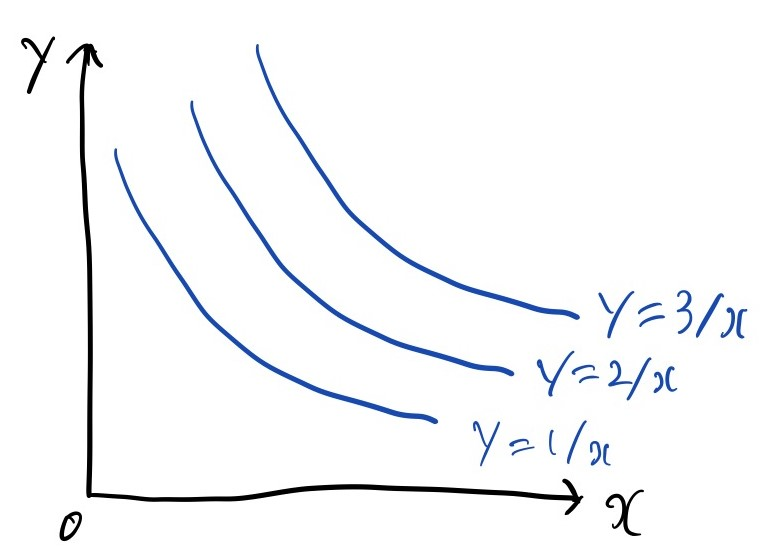
\includegraphics[scale=.3]{pic/IC1.jpg}
            \caption{$y=\frac{i}{x} , i = 1,2,3$}
        \end{figure}
    \end{column}    
    \begin{column}{.5\textwidth}
        \begin{figure}
            \centering
            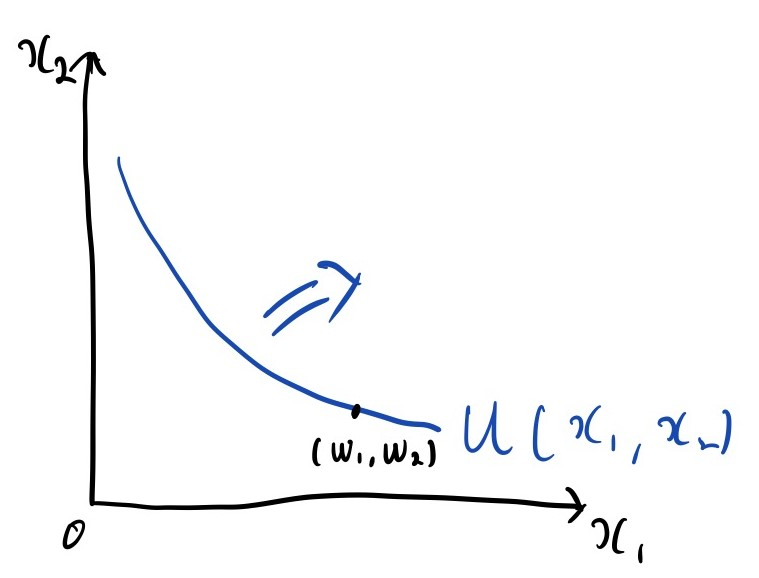
\includegraphics[scale=.3]{pic/IC2.jpg}
            \caption{$U=U(x_1,x_2) = x_1 \times x_2$}
        \end{figure}
    \end{column}    
\end{columns}
\end{frame}
%------------------------------------------------

\begin{frame}{볼록성(Convexity)}
    \begin{figure}
        \centering
        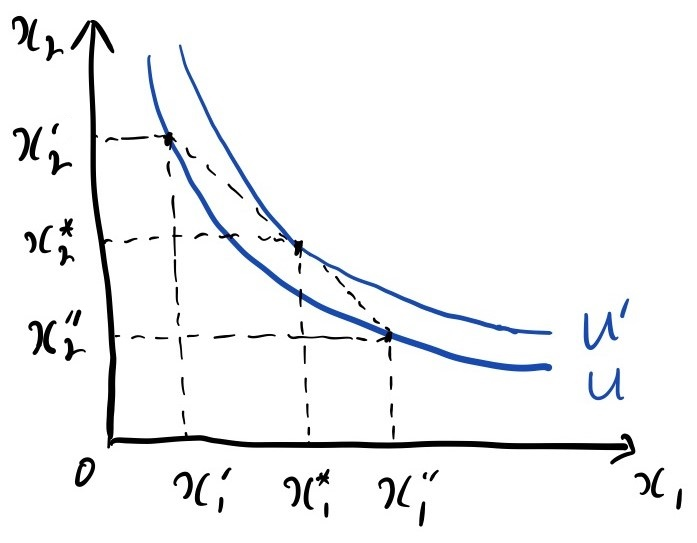
\includegraphics[scale=.3]{pic/convexity.jpg}
        \caption{볼록한 선호}
    \end{figure}
\end{frame}
%------------------------------------------------

\begin{frame}{효용극대화(Utility Maximization)}
\begin{columns}
    \begin{column}{.5\textwidth}
        \begin{figure}
            \centering
            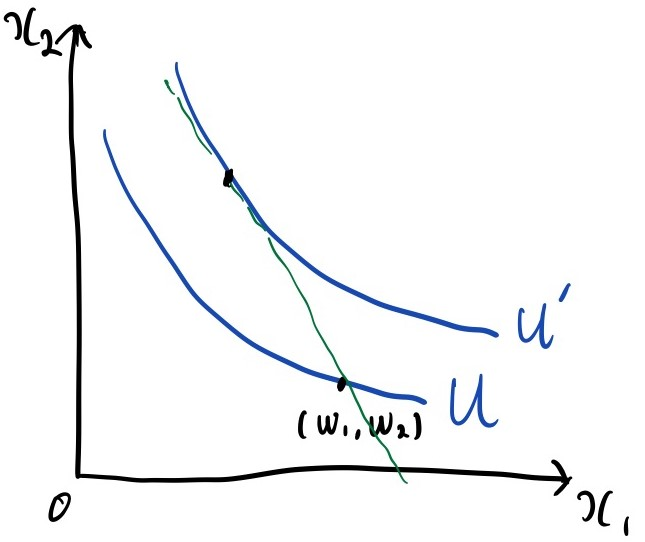
\includegraphics[scale=.3]{pic/umax.jpg}
            \caption{효용극대화}
        \end{figure}
    \end{column}    
    \begin{column}{.5\textwidth}
        \begin{itemize}
            \item 합리적인 소비자는 완전경쟁시장에서 가격이 주어지면(녹색선의 기울기) 자신의 부존자원을 시장을 통해 적절하게 분배하여 자신의 효용을 극대화 한다. 
            \item 이때 자신의 한계 효용은 시장가격과 일치하게 된다.
        \end{itemize}
    \end{column}    
\end{columns}
\end{frame}
%------------------------------------------------

%------------------------------------------------
\section{후생평가의 기준}
%------------------------------------------------

\begin{frame}{후생평가의 기준}
    \begin{itemize}
        \item 사회후생(social welfare)은 한 사회의 (자원분배) 상태를 수치화 한 것.
        \item 사회후생(social welfare)은 구성원들의 효용수준과 직접적인 관계.
        \item 사회후생을 평가하는 주요 기준:
        \begin{itemize}
            \item 효율성(efficiency) : 자원배분의 효율성.
            \item 공평성(equity) : 자원배분의 공평성.
            \item 개인의 자유(right of liberty) : 추가적으로 중요하게 고려해야 할 사항.
        \end{itemize}
        \item 효율성과 공평성이라는 기준의 적용은 현실적으로 많은 어려움이 존재.
        \begin{itemize}
            \item 주로 관점의 차이.
        \end{itemize}
    \end{itemize}
\end{frame}
%------------------------------------------------

%------------------------------------------------
\section{자원배분의 효율성}
%------------------------------------------------

\begin{frame}{효용가능경계(Utility Possibility Frontier)}
    \begin{columns}
        \begin{column}{.5\textwidth}
            \begin{figure}
                \centering
                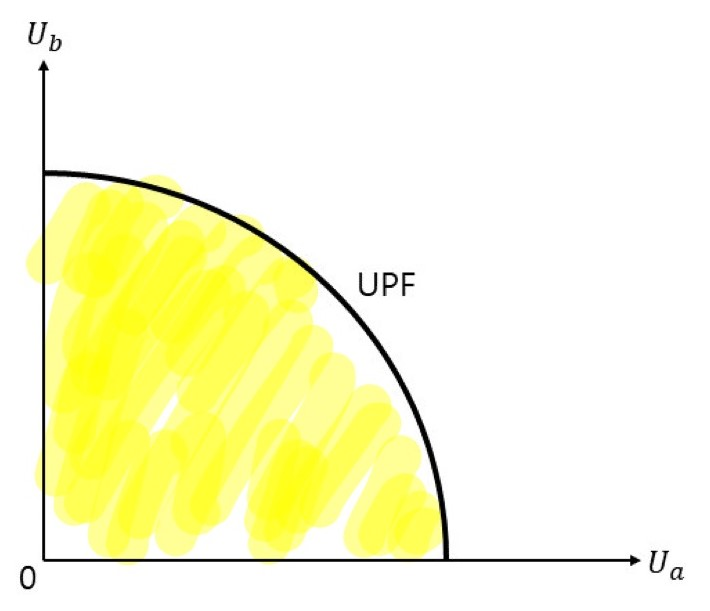
\includegraphics[scale=.3]{pic/UPF.jpg}
                \caption{효용가능경계}
            \end{figure}
        \end{column}    
        \begin{column}{.5\textwidth}
            \begin{itemize}
            \item 순수교환경제(pure exchange economy)에서 효용가능경계(UPF)는 경제에서 효율적 자원 배분이 이루어진 상태의 집합.
            \item 효용가능경계 안쪽(좌하방)의 효용조합은 실현가능하지만 비효울적.
            \end{itemize}
        \end{column}    
    \end{columns}
\end{frame}

\begin{frame}{파레토효율성(Pareto efficiency)}
    \begin{alertblock}{파레토효율성}
        주어진 하나의 자원배분 상태에 대하여, 어느 누구에게도 손해가 가지 않으면서 한 사람 이상에게 이득이 되도록 배분의 변화가 가능하다면 이 변화를 파레토 개선(Pareto improvement)이라고 부른다. 파레토 개선이 불가능한 자원배분은 파레토 효율성을 갖춘 자원배분 이다.
    \end{alertblock}
    \begin{itemize}
        \item 경제학이 의미하는 단 하나의 효율성 개념.
    \end{itemize}
\end{frame}

\begin{frame}{후생경제학 제 1 정리}
    \begin{block}{후생경제학 제 1 정리}
        모든 소비자의 선호체계가 강단조성을 가지면 일반경쟁균형은 파레토 효율적이 된다.
    \end{block}
    \begin{itemize}
        \item 시장의 균형은 효율적이라는 의미.
        \item 아담 스미스(A. Smith)의 보이지 않는 손(invisible hands)의 현대적 해석.
    \end{itemize}
\end{frame}    
%------------------------------------------------

\begin{frame}{에지워스 상자(Edgeworth box)}
    \begin{figure}
        \centering
        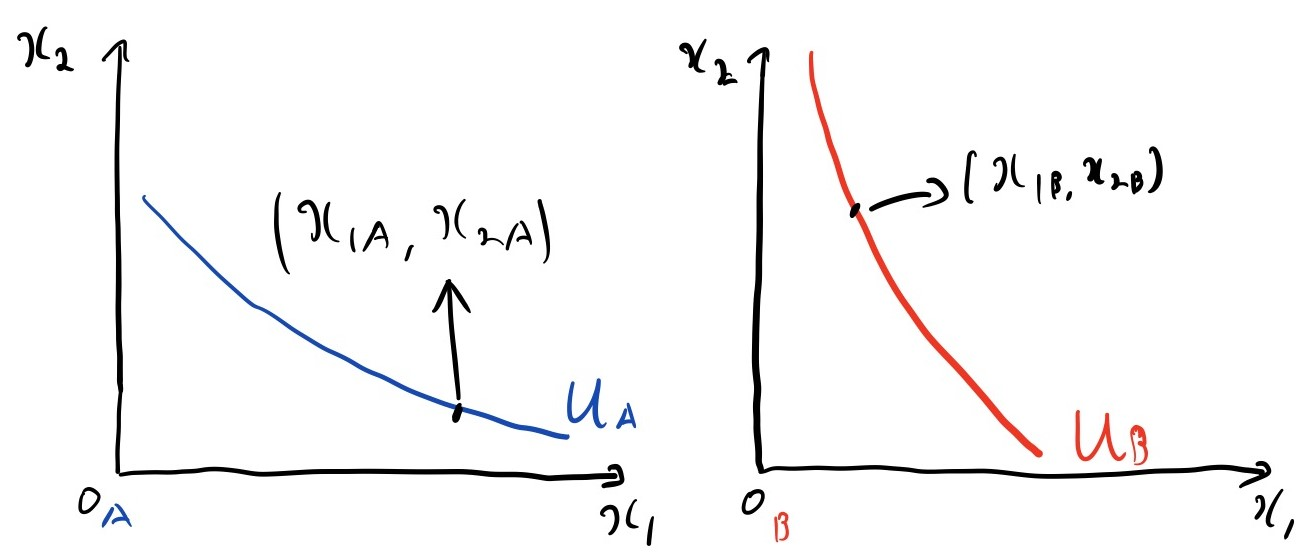
\includegraphics[scale=.35]{pic/2p-1.jpg}
    \end{figure}
\end{frame}
%------------------------------------------------

\begin{frame}{에지워스 상자(Edgeworth box)}
    \begin{figure}
        \centering
        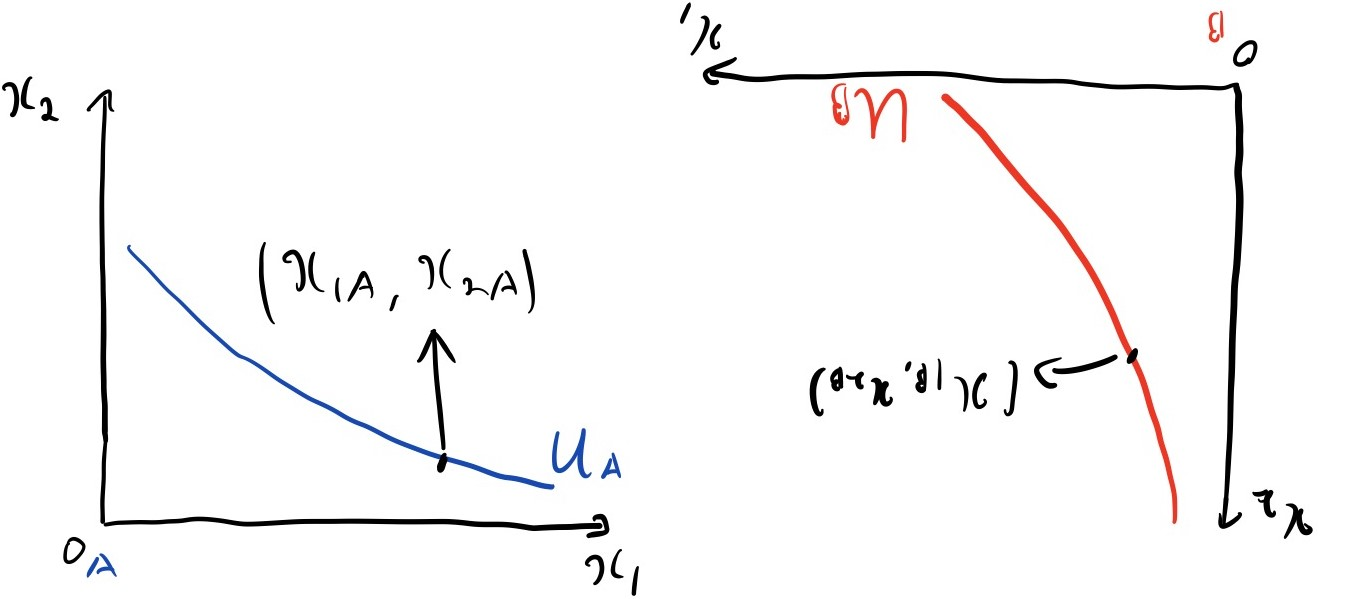
\includegraphics[scale=.35]{pic/2p-2.jpg}
    \end{figure}
\end{frame}
%------------------------------------------------

\begin{frame}{에지워스 상자(Edgeworth box)}
    \begin{figure}
        \centering
        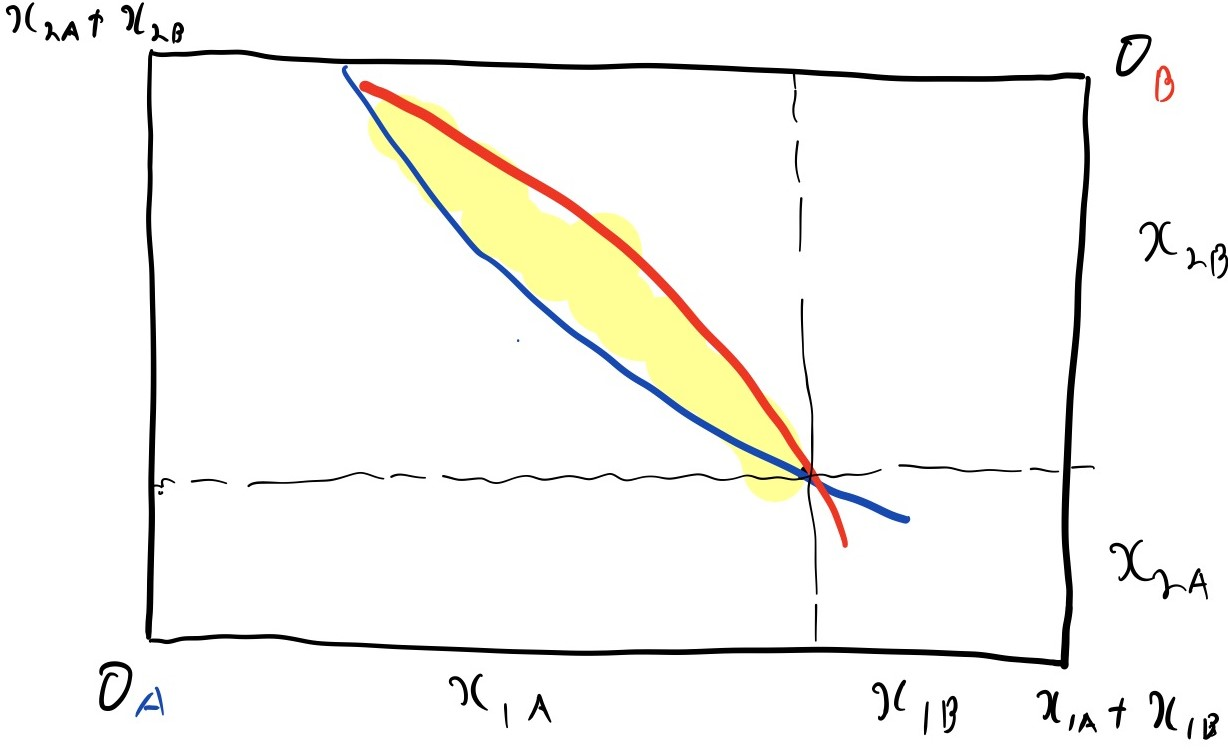
\includegraphics[scale=.3]{pic/box1.jpg}
    \end{figure}
\end{frame}
%------------------------------------------------
\begin{frame}{계약곡선(Contract curve)}
    \begin{figure}
        \centering
        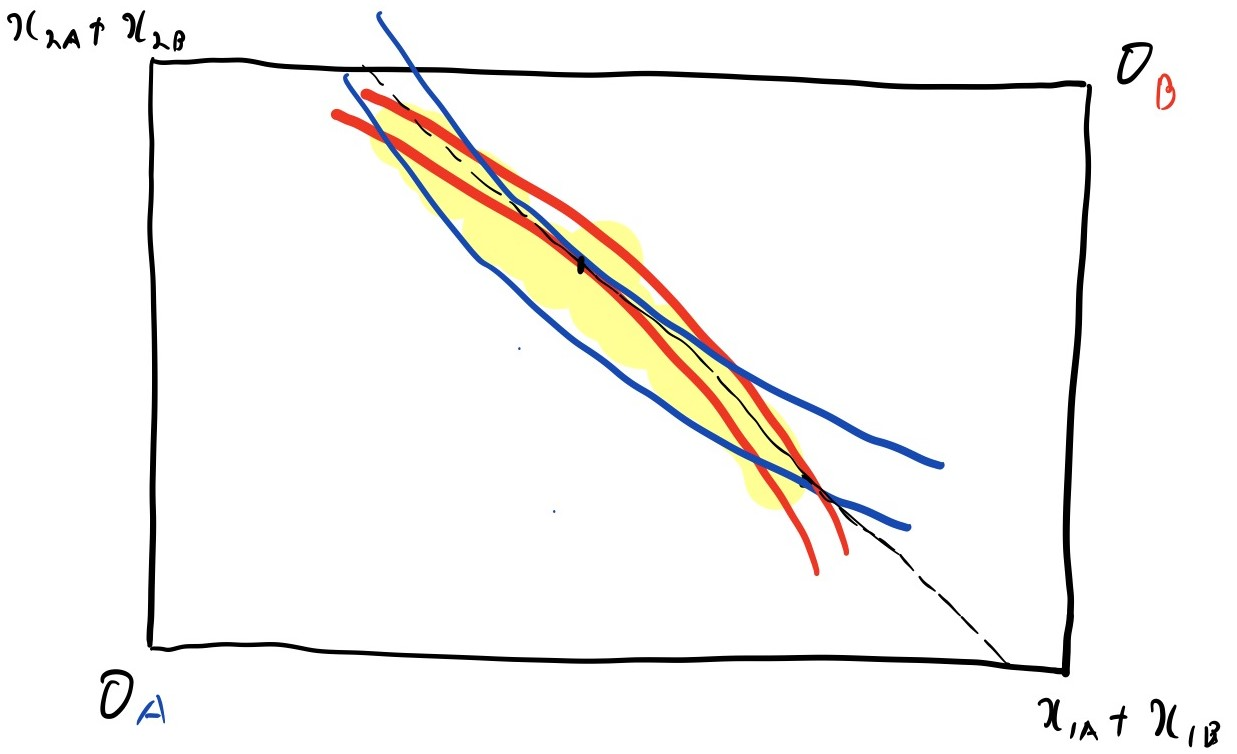
\includegraphics[scale=.3]{pic/box2.jpg}
    \end{figure}
\end{frame}
%------------------------------------------------

\begin{frame}{계약곡선(Contract curve)}
    \begin{figure}
        \centering
        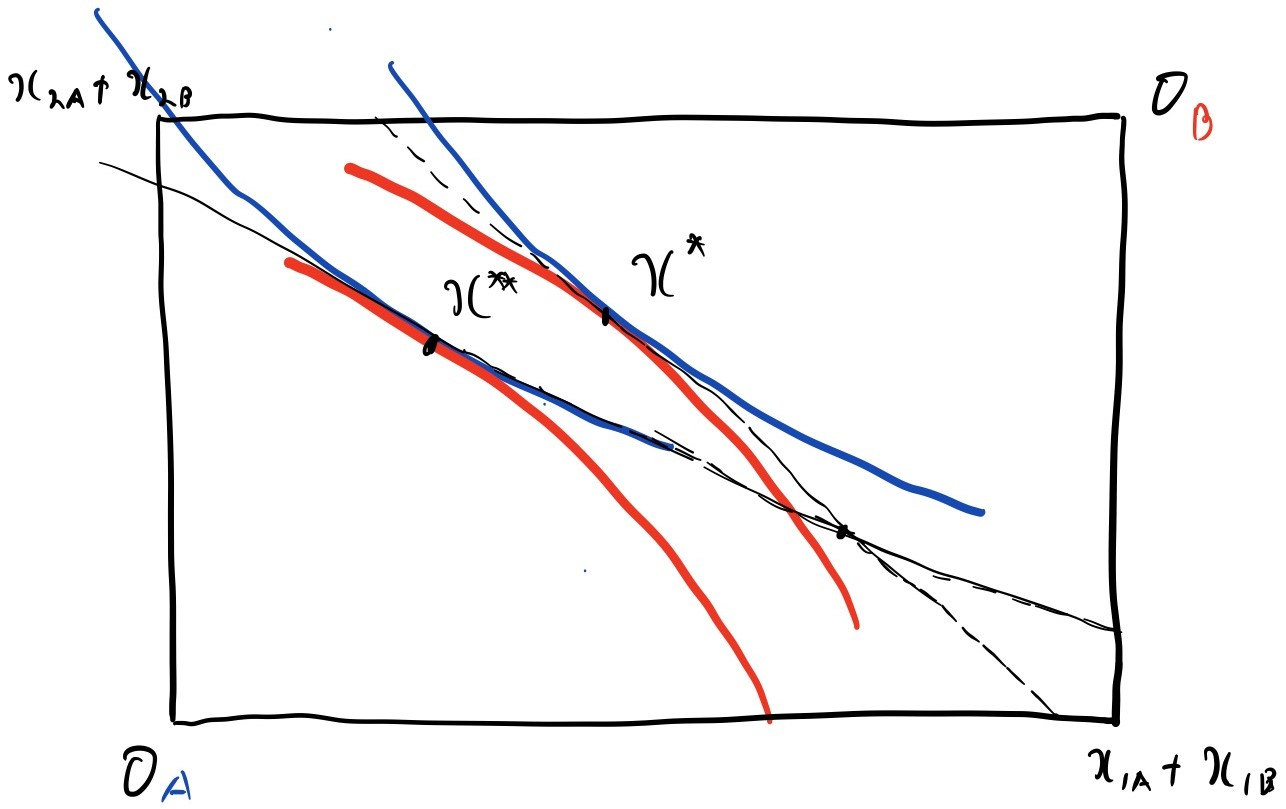
\includegraphics[scale=.3]{pic/contract1.jpg}
    \end{figure}
\end{frame}

%------------------------------------------------
\begin{frame}{계약곡선(Contract curve)}
    \begin{figure}
        \centering
        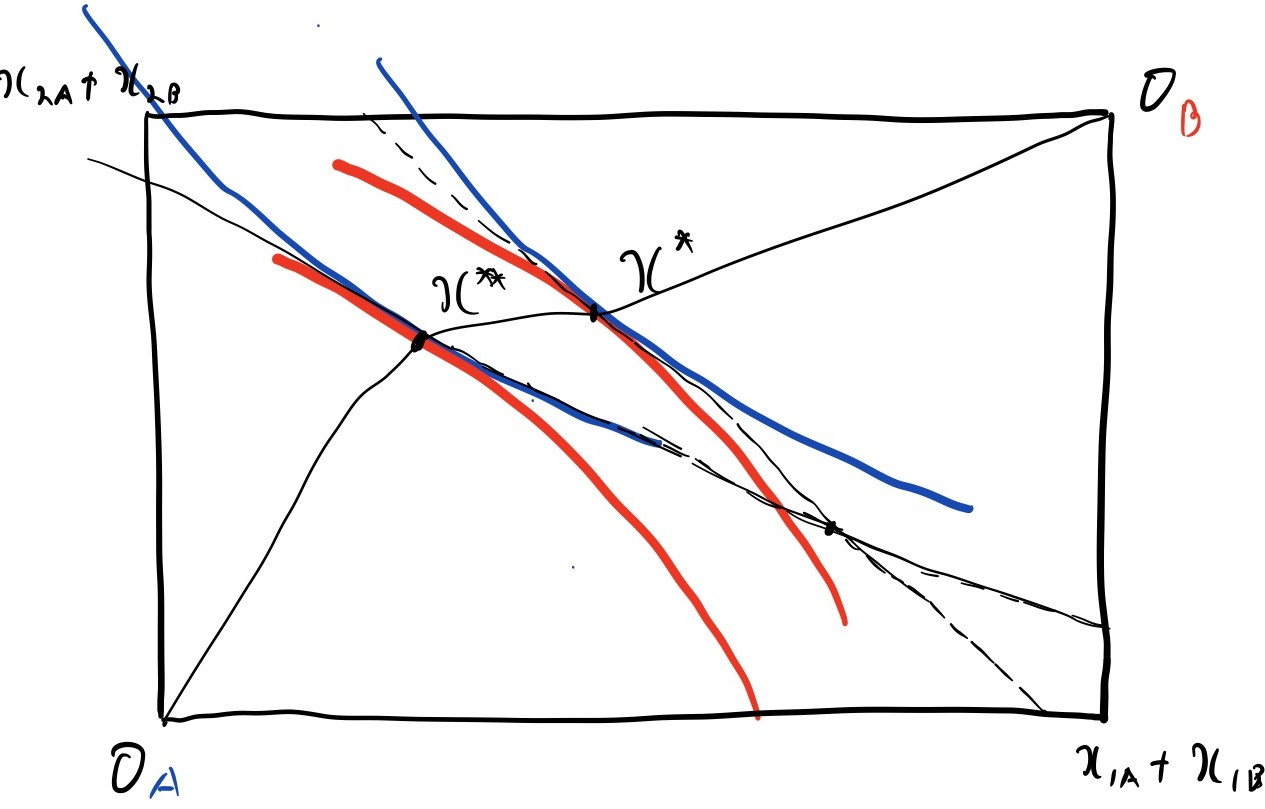
\includegraphics[scale=.3]{pic/contract2.jpg}
    \end{figure}
\end{frame}
%------------------------------------------------
\begin{frame}{후생경제학 제 2 정리}
    \begin{block}{후생경제학 제 2 정리}
        모든 소비자의 선호체계가 볼록성을 가지면, 파레토 효율적인 배분은 초기 부존자원의 적절한 재분배를 통해 일반경쟁균형으로 달성될 수 있다.
    \end{block}
    \begin{itemize}
        \item 모든 효율적인 배분은 시장을 통해 달성 가능하다는 의미.
        \item 효율성의 문제와 재분배의 문제는 분리 가능. 
    \end{itemize}
\end{frame}
%------------------------------------------------

\begin{frame}{재분배}
    \begin{figure}
        \centering
        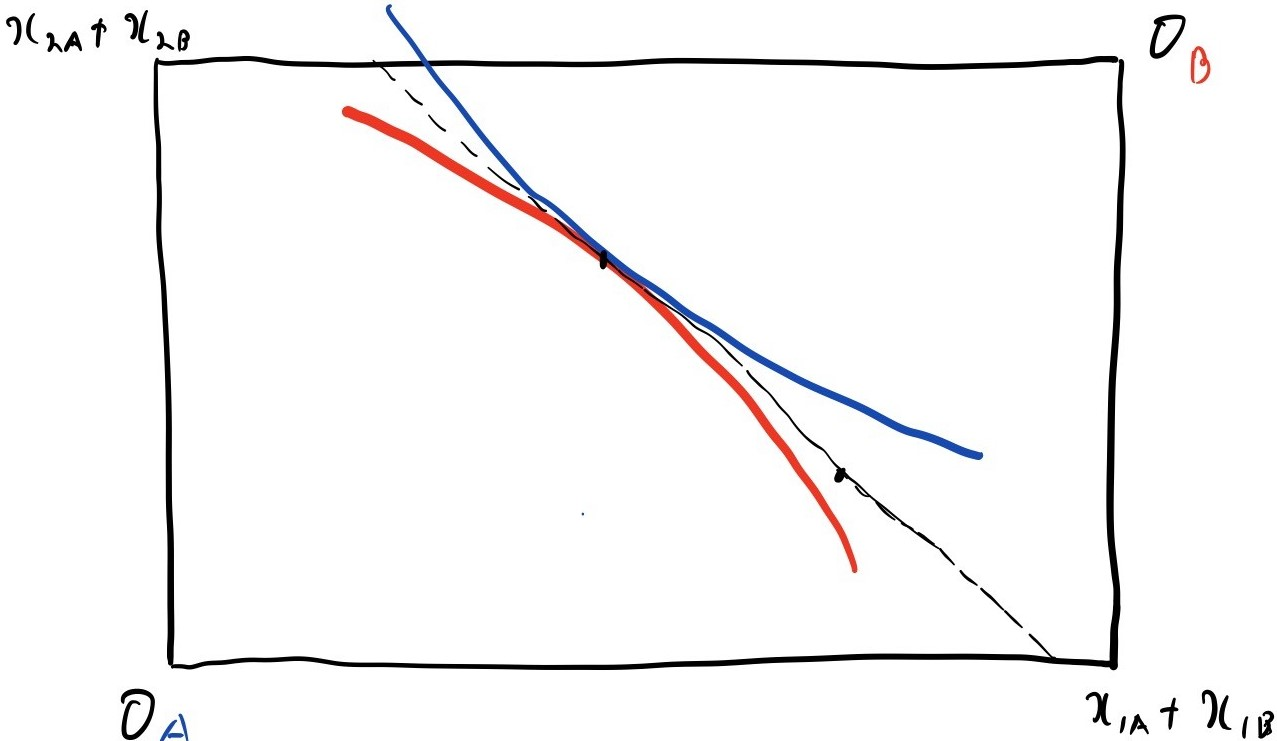
\includegraphics[scale=.3]{pic/trans1.jpg}
    \end{figure}
\end{frame}

\begin{frame}{재분배}
    \begin{figure}
        \centering
        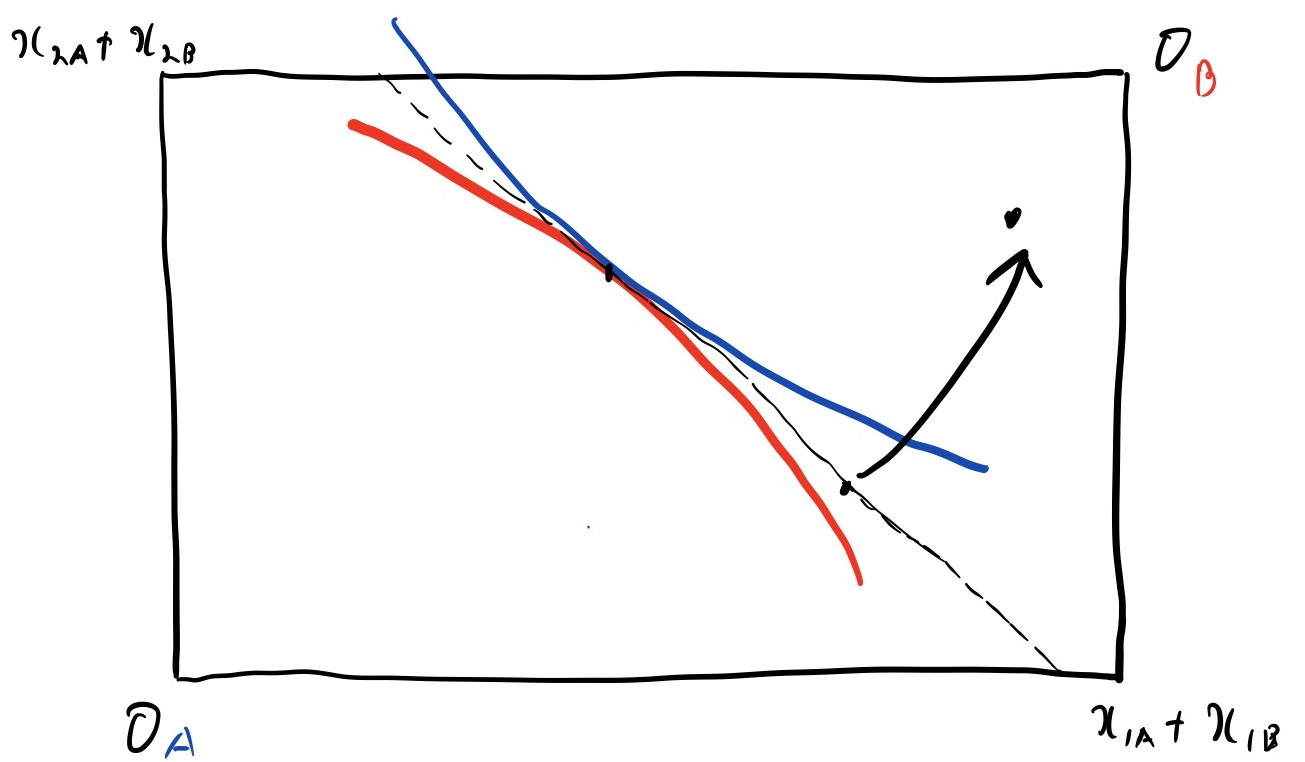
\includegraphics[scale=.3]{pic/trans2.jpg}
    \end{figure}
\end{frame}

\begin{frame}{재분배}
    \begin{figure}
        \centering
        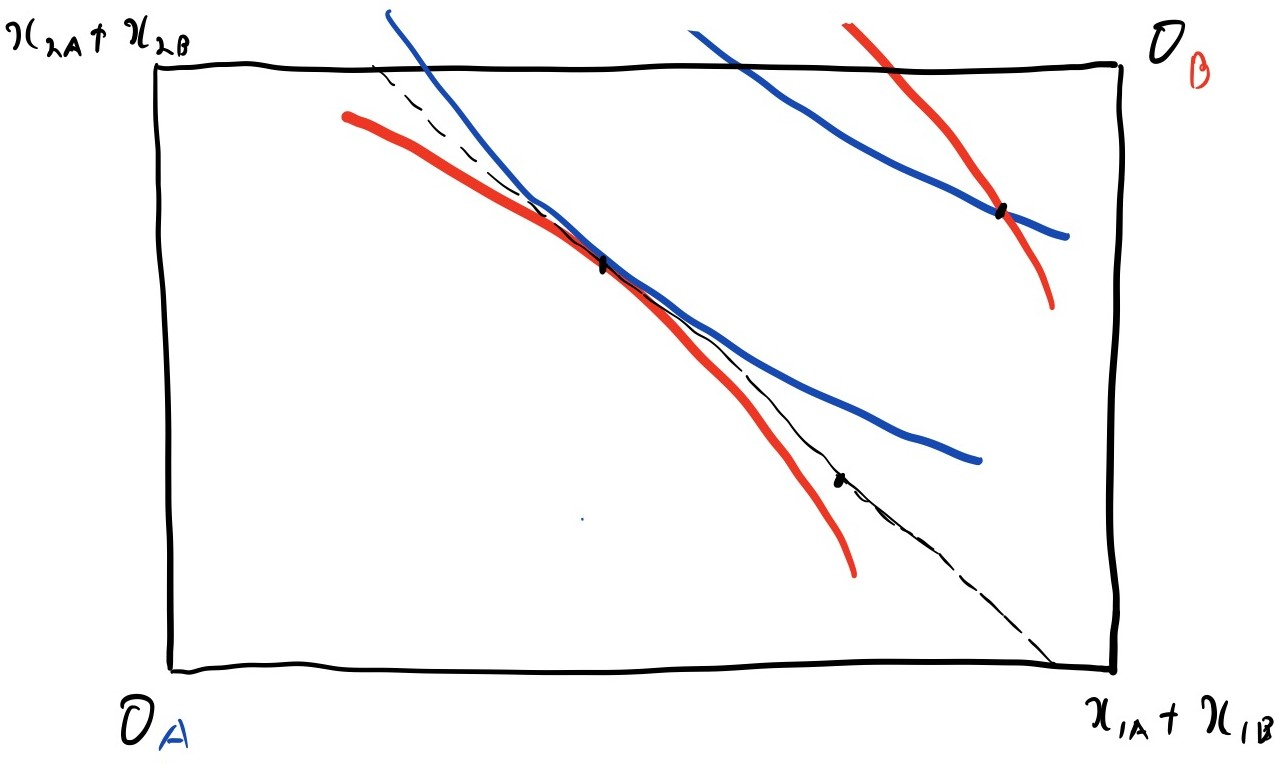
\includegraphics[scale=.3]{pic/trans3.jpg}
    \end{figure}
\end{frame}

\begin{frame}{재분배}
    \begin{figure}
        \centering
        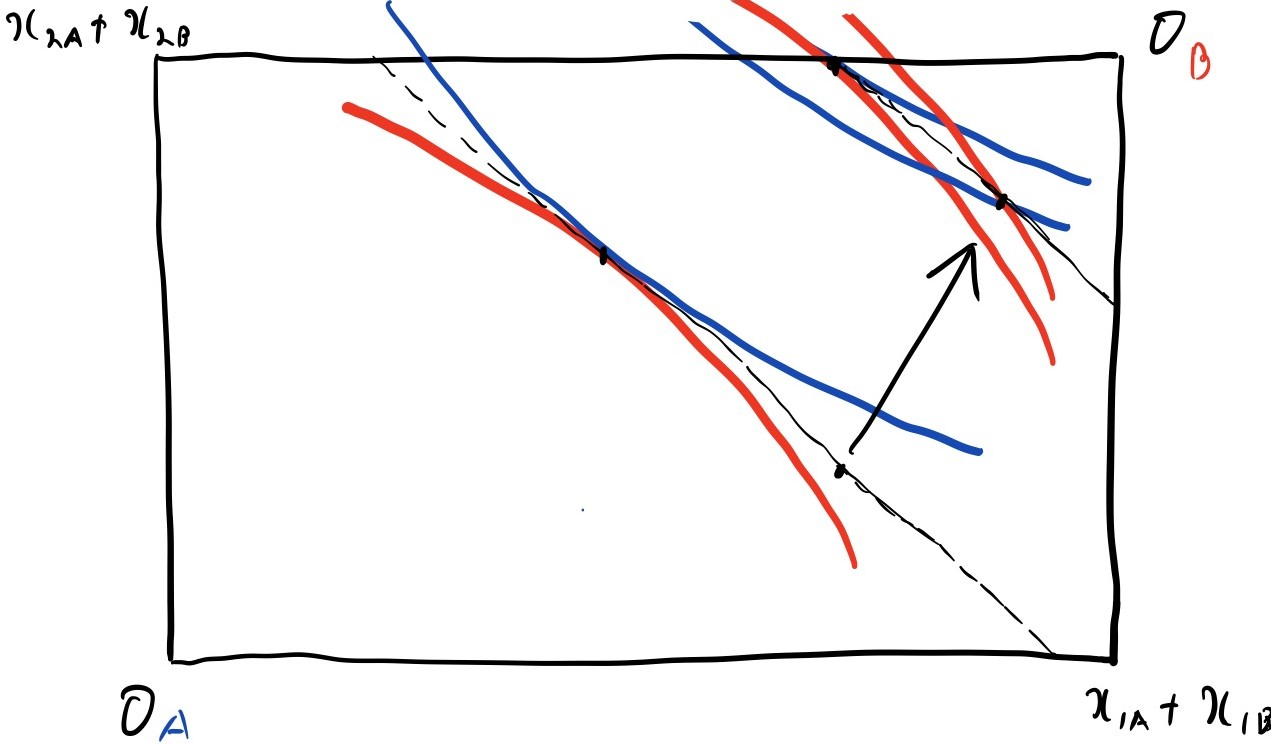
\includegraphics[scale=.3]{pic/trans4.jpg}
    \end{figure}
\end{frame}

%------------------------------------------------
\section{효율적 분배의 실패}
%------------------------------------------------

\begin{frame}{시장실패의 원인I}
    \begin{itemize}
        \begin{alertblock}{완전경쟁시장 }
        무수히 많은 생산자와 소비자가 존재하여 어떤 참여자도 가격에 영향을 줄 수 없는 상태의 시장.
        \end{alertblock}
        \item 불완전경쟁 : 독과점으로 인한 경쟁 저하.
        \item 공공재 :
        \begin{itemize}
            \item 비경합성 : 소비자는 재화 소비를 위해 경쟁하지 않아도 됨.
            \item 배제불가능성 : 재화의 소비에서 타인을 배제할 수 없음.
        \end{itemize}
        \item 외부성 : 한 사람의 행위가 댓가없이 타인에게 영향을 주는 특성 :
        \begin{itemize}
            \item 부정적 영향 : 환경오염, 담배연기, 층간소음 등등.
            \item 긍정적 영향 : 백신접종, 양봉업자와 화훼업자 등등.
        \end{itemize}
    \end{itemize}
\end{frame}

\begin{frame}{시장실패의 원인II}
    \begin{itemize}
        \item 불확실성 : 완벽한 조건부 거래시장(perfect contingency market).
        \item 불완비시장 : 전쟁, 천재지변, 수출입신용, 학자금 등 거래 불가능한 재화.
        \item 불완전정보 :
        \begin{itemize}
            \item 도덕적헤이 : 주인-대리인 문제.
            \item 역선택 : 나쁜 재화가 좋을 재화를 밀어낸다(중고차시장).
        \end{itemize}
        \item 이상의 이유들로 시장은 재화의 효율적 분배에 실패함.
    \end{itemize}
\end{frame}

\begin{frame}{정부의 실패}
    \begin{itemize}
        \item 시장의 실패를 정부가 보완하려는 시도 역시 실패함.
        \begin{itemize}
            \item 제한된 지식과 정보.
            \item 민간부문 반응의 통제 불가능성.
            \item 정치적 과정에서의 제약.
            \item 관료조직에 대한 불완전한 통제.
        \end{itemize}
    \end{itemize}
\end{frame}

%------------------------------------------------
\section{사회후생함수}
%------------------------------------------------
\begin{frame}{보상의 기준}
\begin{columns}
    \begin{column}{.5\textwidth}
        \begin{figure}
            \centering
            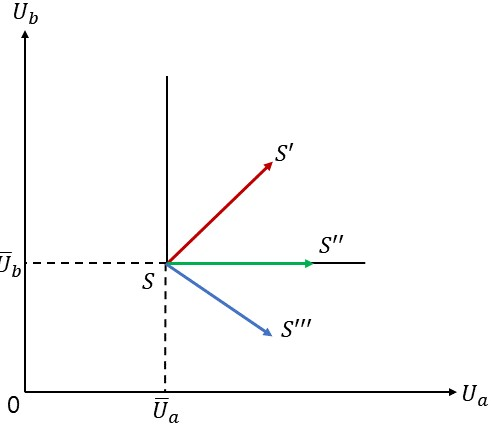
\includegraphics[scale=.4]{pic/Pareto.jpg}
            \caption{파레토 기준}
        \end{figure}
    \end{column}    
    \begin{column}{.5\textwidth}
        \begin{itemize}
            \item 사회후생의 개선여부 기준.
            \item 현실에서 찾기 어려움.
            \item 부자의 1만원 vs. 빈자의 1만원.
            \item 이외에도 칼도, 시코브스키 기준 등이 존재.
        \end{itemize}
    \end{column}    
\end{columns}
\end{frame}



\begin{frame}{사회후생함수(social welfare function)}
    \begin{itemize}
        \item 사회후생의 판단기준으로 기수적 사회후생함수(cardinal SWF)의 도입을 시도.
    \end{itemize}
    \begin{alertblock}{사회후생함수}
        두 사람의 효용수준이 $U_a$, $U_b$로 주어졌을 때, 다음과 같은 관계를 통해 사회후생(social welfare)의 수준을 그 함수값으로 나타내 주는 것을 사회후생함수라고 부른다.
        $$SW = f(U_a, U_b)$$
    \end{alertblock}
    \begin{itemize}
        \item $SW = SW(U_a, U_b)= SW(U_a(x_1,x_2) , U_b(x_1 , x_2))$. 
        \item 사회후생함수의 모양은 주관적 가치판단에 따라 상이.
    \end{itemize}
\end{frame}
%------------------------------------------------

\begin{frame}{공리주의적 사회무차별곡선}
    \begin{figure}
        \centering
        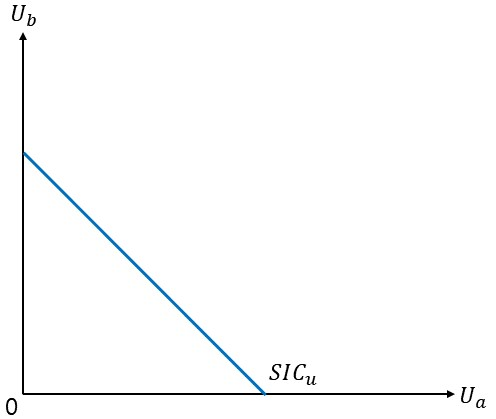
\includegraphics[scale=.4]{pic/Utilitarian.jpg}
        \label{fig:Utilitarian}
    \end{figure}
    \begin{itemize}
       \item $SW=U_a + U_b$.
       \item 두 소비자의 효용의 단순 합만 고려.
    \end{itemize}
\end{frame}
%------------------------------------------------

\begin{frame}{평등주의적 사회무차별곡선}
    \begin{figure}
        \centering
        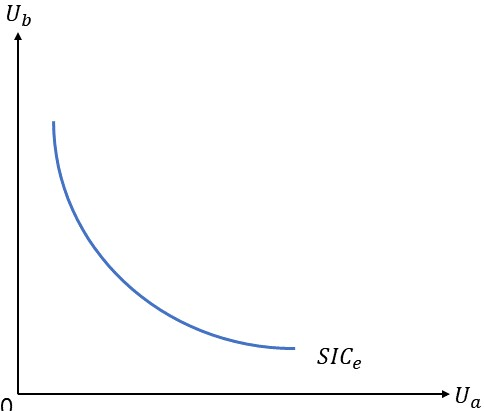
\includegraphics[scale=.4]{pic/Egalitarian.jpg}
        \label{fig:Egalitarian}
    \end{figure}
    \begin{itemize}
       \item $SW=U_a ^\alpha \times U_b ^\beta$.
       \item 개인의 효용이 높아질수록 그 개인의 효용의 사회적 중요도는 하락.
    \end{itemize}
\end{frame}
%------------------------------------------------

\begin{frame}{롤즈적 사회무차별곡선}
    \begin{figure}
        \centering
        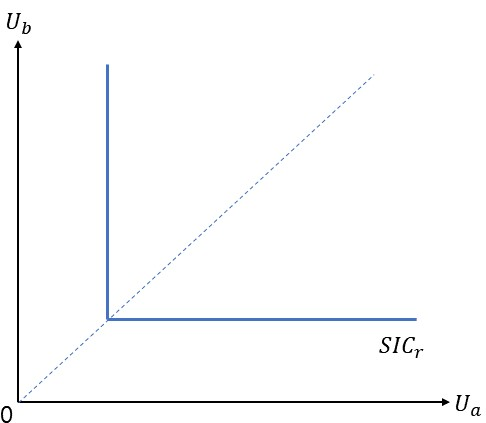
\includegraphics[scale=.4]{pic/Rawlsian.jpg}
        \label{fig:Rawlsian}
    \end{figure}
    \begin{itemize}
        \item $SW = min(U_a, U_b)$.
        \item 사회후생은 개인효용이 가장 낮은 소비자의 수준에서 결정.
    \end{itemize}
\end{frame}
%------------------------------------------------

\begin{frame}{불가능성 정리(Arrow's impossibility theorem)}
    \begin{itemize}
    \item 사회의 선호에 대한 추가 가정
        \begin{itemize}
            \item 무관한 대안으로 부터의 독립 : 대안 A 와 B에 대한 선호는 다른 대안 C에 대한 선호와 무관.
            \item 파레토원칙 : 모든 사람이 A와 B에 대하여 동등하게 선호하면서 적어도 한 명 이상이 A를 좋아한다고 하자. 그러면 사회는 A를 좋아해야 한다. 
        \end{itemize}
    \end{itemize}
    \begin{block}{불가능성정리}
        개인들의 선호가 완비성과 이행성을 만족하는 보편적 상황을 고려하자. \\ 그러면 파레토원칙과 무관한 대안으로부터 독립 그리고 비독재성을 동시에 만족하는 사회후생함수는 존재하지 않는다.
    \end{block}
\end{frame}
%------------------------------------------------

\begin{frame}{결론}
    \begin{itemize}
        \item 경제정의의 문제는 곧 분배적 정의의 문제.
        \item 이상적인 시장기구는 자원배분의 효율성을 달성하지만 현실에서 찾기 어려움.
        \item 효율적이면서 민주적인 이상적인 분배체계는 존재하지 않음.
    \end{itemize}
\end{frame}

%------------------------------------------------

%----------------------------------------------------------------------------------------

\end{document}